\documentclass{article}
\usepackage{amsmath}
\usepackage{mathtools}
\usepackage{graphicx}
\graphicspath{ {images/} }

\title{ECE 742 Final Project}
\author{
  Michelle King
  \and
  Suraj Suri
  }

\begin{document}
\maketitle
\section{Theory}
\subsection{PML}
Perfectly Matched Layer (PML) boundary conditions are absorbing boundary
conditions. PML BCs decay the wave within a boundary layer at the edge of the
simulation. The edge of the simulation BC can be implemented as PEC.
Well-implemented PML BCs completely decay the wave from the time it enters the
boundary layer to the time after it reflects and attempts to leave.

\subsection{Finite-Difference Derivation}
Let's start with equation:
\begin{equation}\nabla \times \vec{H} = j \omega \epsilon \bar{\bar{s}} \vec{E}\end{equation}
Evaluate the cross product and write in matrix form:
\begin{equation}
  $
  \begin{bmatrix}
    \frac{\partial H_{z}}{\partial y}-\frac{\partial H_{y}}{\partial z} \\
    \frac{\partial H_{x}}{\partial z}-\frac{\partial H_{z}}{\partial x} \\
    \frac{\partial H_{y}}{\partial x}-\frac{\partial H_{x}}{\partial y}
  \end{bmatrix}
  =
  j\omega\epsilon
  \begin{bmatrix}
    \frac{s_{y}s_{z}}{s_{x}} & 0                       & 0                       \\
    0                       & \frac{s_{x}s_{z}}{s_{y}} & 0                       \\
    0                       & 0                       & \frac{s_{x}s_{y}}{s_{z}} \\
  \end{bmatrix}
  \begin{bmatrix}
    E_{x} \\
    E_{y} \\
    E_{z}
  \end{bmatrix}
  $
\end{equation}
Where the values in the second rank tensor can be described by:
\begin{equation}s_{x}=\kappa_{x}+\frac{\sigma_{x}}{j\omega\epsilon_{0}}\end{equation}
\begin{equation}s_{y}=\kappa_{y}+\frac{\sigma_{y}}{j\omega\epsilon_{0}}\label{SyEquation}\end{equation}
\begin{equation}s_{z}=\kappa_{z}+\frac{\sigma_{z}}{j\omega\epsilon_{0}}\label{SzEquation}\end{equation}
To make the calculation computationally more managable, we can define the following
relations:
\begin{equation}D_{x}=\epsilon \frac{s_{z}}{s_{x}}E_{x}\end{equation}
\begin{equation}D_{y}=\epsilon \frac{s_{x}}{s_{y}}E_{y}\end{equation}
\begin{equation}D_{z}=\epsilon \frac{s_{y}}{s_{z}}E_{z}\label{DzEzRelation}\end{equation}
such that now:
\begin{equation}
  $
  \begin{bmatrix}
    \frac{\partial H_{z}}{\partial y}-\frac{\partial H_{y}}{\partial z} \\
    \frac{\partial H_{x}}{\partial z}-\frac{\partial H_{z}}{\partial x} \\
    \frac{\partial H_{y}}{\partial x}-\frac{\partial H_{x}}{\partial y}
  \end{bmatrix}
  =
  j\omega
  \begin{bmatrix}
    s_{y}  & 0      & 0     \\
    0      & s_{z}  & 0     \\
    0      & 0     & s_{x}  \\
  \end{bmatrix}
  \begin{bmatrix}
    D_{x} \\
    D_{y} \\
    D_{z}
  \end{bmatrix}
  $
\end{equation}
Using the defined values of s and that $\frac{\partial}{\partial t} = j \omega $:
\begin{equation}
  $
  \begin{bmatrix}
    \frac{\partial H_{z}}{\partial y}-\frac{\partial H_{y}}{\partial z} \\
    \frac{\partial H_{x}}{\partial z}-\frac{\partial H_{z}}{\partial x} \\
    \frac{\partial H_{y}}{\partial x}-\frac{\partial H_{x}}{\partial y}
  \end{bmatrix}
  $
  =
  \frac{\partial}{\partial t}
  $
  \begin{bmatrix}
    \kappa_{y}  & 0           & 0           \\
    0           & \kappa_{z}  & 0           \\
    0           & 0           & \kappa_{x}  \\
  \end{bmatrix}
  \begin{bmatrix}
    D_{x} \\
    D_{y} \\
    D_{z}
  \end{bmatrix}
  $
  +\frac{1}{\epsilon_{0}}
  $
  \begin{bmatrix}
    \sigma_{y}  & 0           & 0           \\
    0           & \sigma_{z}  & 0           \\
    0           & 0           & \sigma_{x}  \\
  \end{bmatrix}
  \begin{bmatrix}
    D_{x} \\
    D_{y} \\
    D_{z}
  \end{bmatrix}
  $
\end{equation}

This has too much info. Since we are doing 2D, $\kappa_{z}=1$, $\sigma_{z}=0$ in
this simulation. We are doing TM as well, so $D_{x}=D_{y}=0$ and $H_{z}=0$. Equation reduces to:

\begin{equation}
  $
  \begin{bmatrix}
    \frac{\partial H_{z}}{\partial y}-\frac{\partial H_{y}}{\partial z} \\
    \frac{\partial H_{x}}{\partial z}-\frac{\partial H_{z}}{\partial x} \\
    \frac{\partial H_{y}}{\partial x}-\frac{\partial H_{x}}{\partial y}
  \end{bmatrix}
  $
  =
  \frac{\partial}{\partial t}
  $
  \begin{bmatrix}
    \kappa_{y}  & 0   & 0          \\
    0           & 1   & 0           \\
    0           & 0   & \kappa_{x}   \\
  \end{bmatrix}
  \begin{bmatrix}
    0 \\
    0 \\
    D_{z}
  \end{bmatrix}
  $
  +\frac{1}{\epsilon_{0}}
  $
  \begin{bmatrix}
    \sigma_{y}  & 0  & 0           \\
    0           & 0  & 0           \\
    0           & 0  & \sigma_{x}   \\
  \end{bmatrix}
  \begin{bmatrix}
    0 \\
    0 \\
    D_{z}
  \end{bmatrix}
  $
\end{equation}

This leaves us with one equation to find an update quation for  $D_{z}$:
\begin{equation}
  \frac{\partial H_{y}}{\partial x}-\frac{\partial H_{x}}{\partial y}=  \kappa_{x}\frac{\partial}{\partial t} D_{z}+\frac{\sigma_{x}}{\epsilon_{0}} D_{z}
\end{equation}


Using semi-implicit definition

\begin{equation}D^{n+1/2}=\frac{D^{n+1}+D^{n}}{2}\end{equation}

If we discretize around point i,j,k at timestep n

This equation discretizes to:

\begin{equation}
\begin{multlined}
  \frac{1}{\Delta_{x}}(H_{y}^{n+1/2}(i+1/2,j)-H_{y}^{n+1/2}(i-1/2,j)) \\
 -\frac{1}{\Delta_{y}}(H_{x}^{n+1/2}(i,j+1/2)-H_{x}^{n+1/2}(i,j-1/2))= \\
  \frac{\kappa_{x}}{\Delta t}
   (D_{z}^{n+1}(i,j)-D_{z}^{n}(i,j))+
   \frac{\sigma_{x}}{2 \epsilon_{0}}
   (D_{z}^{n+1}(i,j)+D_{z}^{n}(i,j))
\end{multlined}
\end{equation}


 We can solve this to find update equation for D:

\begin{equation}
\begin{multlined}
  \frac{1}{\Delta_{x}}(H_{y}^{n+1/2}(i+1/2,j)-H_{y}^{n+1/2}(i-1/2,j)) \\
 -\frac{1}{\Delta_{y}}(H_{x}^{n+1/2}(i,j+1/2)-H_{x}^{n+1/2}(i,j-1/2))= \\
  (\frac{\sigma_{x}}{2\epsilon_{0}}+\frac{\kappa_{x}}{\Delta t})D_{z}^{n+1}(i,j)+
  (\frac{\sigma_{x}}{2\epsilon_{0}}-\frac{\kappa_{x}}{\Delta t})D_{z}^{n}(i,j)
\end{multlined}
\end{equation}

\begin{equation}
\begin{multlined}
  \frac{1}{\Delta_{x}}(H_{y}^{n+1/2}(i+1/2,j)-H_{y}^{n+1/2}(i-1/2,j)) \\
 -\frac{1}{\Delta_{y}}(H_{x}^{n+1/2}(i,j+1/2)-H_{x}^{n+1/2}(i,j-1/2))= \\
  (\frac{\sigma_{x}\Delta t+2\epsilon_{0}\kappa_{x}}{2\epsilon_{0}\Delta t})D_{z}^{n+1}(i,j)+
  (\frac{\sigma_{x}\Delta t-2\epsilon_{0}\kappa_{x}}{2\epsilon_{0}\Delta t})D_{z}^{n}(i,j)
\end{multlined}
\end{equation}

\begin{equation}
\begin{multlined}
  D_{z}^{n+1}(i,j) = -\frac{\sigma_{x}\Deltat-2\epsilon_{0}\kappa_{x}}{\sigma_{x}\Delta t+2\epsilon_{0}\kappa_{x}}D_{z}^{n}(i,j) \\
  +\frac{2\epsilon_{0}\Delta t}{\Delta_{x}(\sigma_{x}\Delta t+2\epsilon_{0}\kappa_{x})}(H_{y}^{n+1/2}(i+1/2,j)-H_{y}^{n+1/2}(i-1/2,j)) \\
 -\frac{2\epsilon_{0}\Delta t}{\Delta_{y}(\sigma_{x}\Delta t+2\epsilon_{0}\kappa_{x})}(H_{x}^{n+1/2}(i,j+1/2)-H_{x}^{n+1/2}(i,j-1/2))
\end{multlined}
\end{equation}

 
 Update Components for E\\

 Start with rewriting \ref{DzEzRelation}:
 \begin{equation}s_{z}D_{z}=\epsilon s_{y}E_{z}\end{equation}

 Using \ref{SyEquation} and \ref{SzEquation}:

 \begin{equation}(\kappa_{z}+\frac{\sigma_{z}}{j\omega\epsilon_{0}})D_{z}=\epsilon
   (\kappa_{y}+\frac{\sigma_{y}}{j\omega\epsilon_{0}})E_{z}\end{equation}

 Take the partial time derivative and use $\frac{\partial}{\partial t}= j \omega$
 
 \begin{equation}
   \frac{\partial}{\partial t}(\kappa_{z}D_{z})+\frac{\sigma_{z}}{\epsilon_{0}}D_{z}=
   \epsilon(\frac{\partial}{\partial t}(\kappa_{y}E_{z})+\frac{\sigma_{y}}{\epsilon_{0}}E_{z})
 \end{equation}

 Discretize this to find update equation for E:

 \begin{equation}
 E_{z}^{n+1}(i,j) = \frac{2\epsilon_{0}\kappa_{y}-\sigma_{y}\Delta t}{2\epsilon_{0}\kappa_{y}+\sigma_{y}\Delta t} E_{z}^{n}(i,j)+\frac{1}{2\epsilon_{0}\kappa_{y}+\sigma_{y}\Delta t}  ((2\epsilon_{0}\kappa_{z}+\sigma_{z}\Delta t) D_{z}^{n+1}(i,j)-(2\epsilon_{0}\kappa_{z}-\sigma_{z}\Delta t) D_{y}^{n}(i,j))/\epsilon
 \end{equation}
 
 Similarly, we can find the B update equations to be:

 \begin{equation}
 B_{x}^{n+1/2}(i,j) = \frac{2\epsilon_{0}\kappa_{y}-\sigma_{y}\Delta t}{2\epsilon_{0}\kappa_{y}+\sigma_{y}\Delta t}  B_{x}^{n-1/2}(i,j) + \frac{2\epsilon_{0}\Delta t}{2\epsilon_{0}\kappa_{y}+\sigma_{y}\Delta t}  (E_{z}^{n}(i,j+1)-E_{z}^{n}(i,j))/dy
 \end{equation}
 \begin{equation}
 B_{y}^{n+1/2}(i,j) = \frac{2\epsilon_{0}\kappa_{z}-\sigma_{z}\Delta t}{2\epsilon_{0}\kappa_{z}+\sigma_{z}\Delta t}  B_{y}^{n-1/2}(i,j) + \frac{2\epsilon_{0}\Delta t}{2\epsilon_{0}\kappa_{z}+\sigma_{z}\Delta t}  (E_{z}^{n}(i+1,j)-E_{z}^{n}(i,j))/dx
 \end{equation}

 And we can find the H update equations to be:

 \begin{equation}
 H_{x}^{n+1}(i,j) = \frac{2\epsilon_{0}\kappa_{z}-\sigma_{z}\Delta t}{2\epsilon_{0}\kappa_{z}+\sigma_{z}\Delta t}  H_{x}^{n}(i,j) + \frac{1}{2\epsilon_{0}\kappa_{z}+\sigma_{z}\Delta t}  ((2\epsilon_{0}\kappa_{x}+\sigma_{x}\Delta t) B_{x}^{n+1}(i,j)-(2\epsilon_{0}\kappa_{x}-\sigma_{x}\Delta t) B_{x}^{n}(i,j))/\mu
 \end{equation}
 \begin{equation}
 H_{y}^{n+1}(i,j) = \frac{2\epsilon_{0}\kappa_{x}-\sigma_{x}\Delta t}{2\epsilon_{0}\kappa_{x}+\sigma_{x}\Delta t}  H_{y}^{n}(i,j) + \frac{1}{2\epsilon_{0}\kappa_{x}+\sigma_{x}\Delta t}  ((=2\epsilon_{0}\kappa_{y}+\sigma_{y}\Delta t) B_{y}^{n+1}(i,j)-(2\epsilon_{0}\kappa_{y}\sigma_{y}\Delta t) B_{y}^{n}(i,j))/\mu
 \end{equation} 

\subsection{Code Implementation}
\subsubsection{Update Equations}
 Using the derivation above, we can update field values in a loop. It is
 computationally more efficient to calculate the coefficients for these field
 values as an array outside of the loop. This gives us 18 coefficients and their
 corresponding simplified field update equations:
 \begin{equation}
   Ez
 \end{equation}
 \begin{equation}
   CBX1=\frac{2\epsilon_{0}\kappa_{y}-\sigma_{y}\Delta t}{2\epsilon_{0}\kappa_{y}+\sigma_{y}\Delta t}
 \end{equation}
 \begin{equation}
   CBX2=\frac{2\epsilon_{0}\Delta t}{2\epsilon_{0}\kappa_{y}+\sigma_{y}\Delta t}
 \end{equation}
 \begin{equation}
   CHX1=\frac{2\epsilon_{0}\kappa_{z}-\sigma_{z}\Delta t}{2\epsilon_{0}\kappa_{z}+\sigma_{z}\Delta t}
 \end{equation}
 \begin{equation}
   CHX2=\frac{1}{2\epsilon_{0}\kappa_{z}+\sigma_{z}\Delta t}
 \end{equation}
 \begin{equation}
   CHX3=2\epsilon_{0}\kappa_{x}+\sigma_{x}\Delta t
 \end{equation}
  \begin{equation}
   CHX4=2\epsilon_{0}\kappa_{x}-\sigma_{x}\Delta t
 \end{equation}

 \begin{equation}
   CBY1=\frac{2\epsilon_{0}\kappa_{z}-\sigma_{z}\Delta t}{2\epsilon_{0}\kappa_{z}+\sigma_{z}\Delta t}
 \end{equation}
 \begin{equation}
   CBY2=\frac{2\epsilon_{0}\Delta t}{2\epsilon_{0}\kappa_{z}+\sigma_{z}\Delta t}
 \end{equation}
 \begin{equation}
   CHY1=\frac{2\epsilon_{0}\kappa_{x}-\sigma_{x}\Delta t}{2\epsilon_{0}\kappa_{x}+\sigma_{x}\Delta t}
 \end{equation}
 \begin{equation}
   CHY2=\frac{1}{2\epsilon_{0}\kappa_{x}+\sigma_{x}\Delta t}
 \end{equation}
 \begin{equation}
   CHY3=2\epsilon_{0}\kappa_{y}+\sigma_{y}\Delta t
 \end{equation}
  \begin{equation}
   CHY4=2\epsilon_{0}\kappa_{y}-\sigma_{y}\Delta t
 \end{equation}
  \begin{equation}
   CDZ1=\frac{2\epsilon_{0}\kappa_{x}-\sigma_{x}\Delta t}{2\epsilon_{0}\kappa_{x}+\sigma_{x}\Delta t}
 \end{equation}
 \begin{equation}
   CDZ2=\frac{2\epsilon_{0}\Delta t}{2\epsilon_{0}\kappa_{x}+\sigma_{x}\Delta t}
 \end{equation}
 \begin{equation}
   CEZ1=\frac{2\epsilon_{0}\kappa_{y}-\sigma_{y}\Delta t}{2\epsilon_{0}\kappa_{y}+\sigma_{y}\Delta t}
 \end{equation}
 \begin{equation}
   CEZ2=\frac{1}{2\epsilon_{0}\kappa_{y}+\sigma_{y}\Delta t}
 \end{equation}
 \begin{equation}
   CEZ3=2\epsilon_{0}\kappa_{z}+\sigma_{z}\Delta t
 \end{equation}
  \begin{equation}
   CEZ4=2\epsilon_{0}\kappa_{z}-\sigma_{z}\Delta t
 \end{equation}

 Some of these coefficients are identical, but we stored them separately for the
 purpose of organization and readable naming scheme.
 
\subsubsection{Graded PML}
The purpose of PML is to have the wave decay as the wave enters the PML, and a
nonzero conductivity value will achieve this decay. However, a large discrepancy
between the values of conductivity in the simulation region and the PML can
result in unwanted reflections.

The Reflection Factor is given by the equation:
\begin{equation}
  R(\theta)=\exp^{-2\eta cos(\theta)\int_{0}^{d}\sigma_{x}(x)dx
\end{equation}

  Where $\sigma_{x}$ is the graded conductivity of the PML material.\\
  $\theta$ is the angle of incidence of the wave. So steeper angles of $\theta$
  will result in higher values of reflection error.\\
  
We want to minimize reflection R but also make sure the wave decays completely
within the PML.

\subsubsection{Polynomial grading}
One type of grading, and the one  we have implemented, is the polynomial grading. We can
describe the grading in our code by the factors $\sigma$ and $\kappa$
Where the graded conductivity for the PML in the x direction is:
\[\sigma_{x} = (\frac{x}{d})^{m} \sigma_{x,max}\]
And the graded value for $\kappa$ for the PML in the x direction is:
\[\kappa_{x}=1+(\kappa_{x,max}-1)(\frac{x}{d})^{m}\]

We will vary the values for $\kappa_{max}$ and $\sigma_{max}$ in our numerical
experiments to test how different PML material conditions affect the
effectiveness of the PML.

An optimal expression for the value of $\sigma_{max}$ for a polynomial grading
has been found numerically to be:
\begin{equation}
\sigma_{x, optimal}=\frac{0.8(m+1)}{\eta_{0} \Delta x}
\end{equation}

\section{Experiment}
Each E and H componenet within the UPML is computed using a two-step 


We varied values of sig this tells us _____

We varied ____ this tells us ____

We varied _____ this tells us _____


\section{Error Analysis}
In order to test how well the PML is working to absorb the incoming reflection,
we will calculate the relative error with respect to the case of no boundary
conditions. Error values were calculated for the amount of the wave within the
simulation region, not including the wave present in the PML.  

\begin{figure}
  \centering
  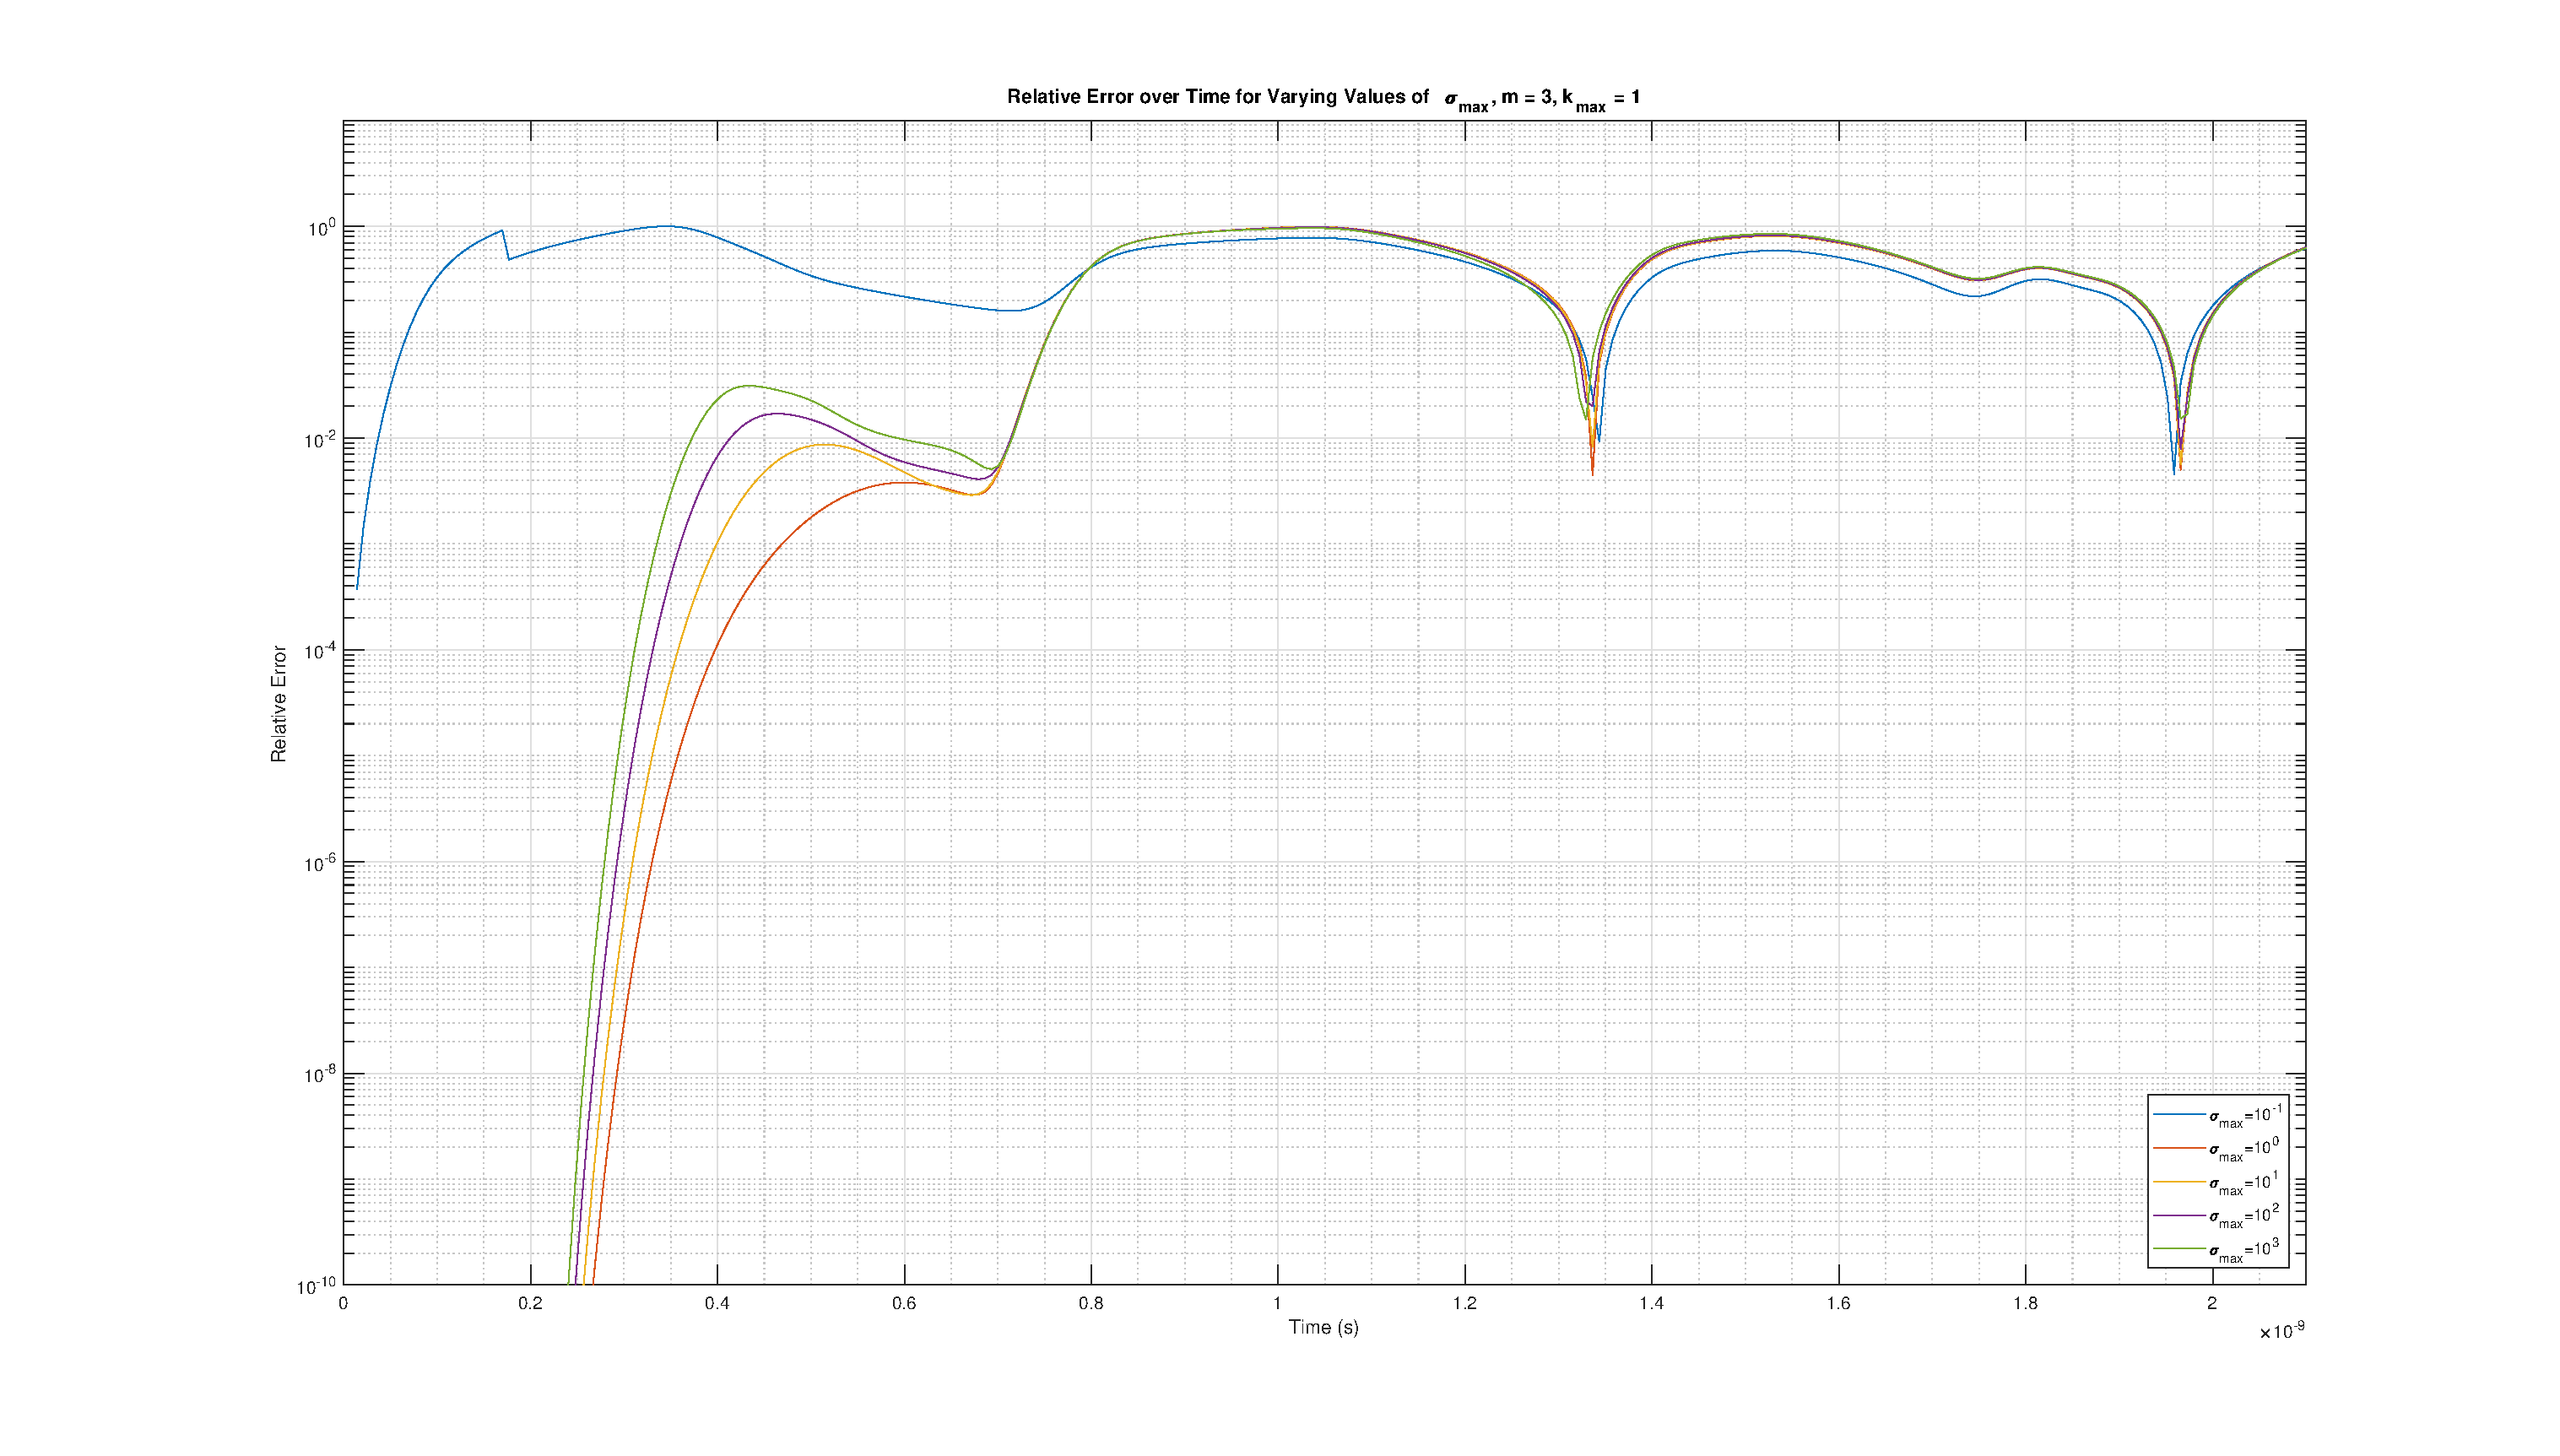
\includegraphics[width=\textwidth]{Rel_Err_SigMax_m3}
  \caption{Plot of Relative Error with respect to time for values of
    \sigma_{max} of 10^{-1}, 10^0, 10^1, 10^2, 10^3, m=3, \kappa{max}=3}\label{fig:RelErrSigmaxm3}
\end{figure}


\begin{figure}
  \centering
  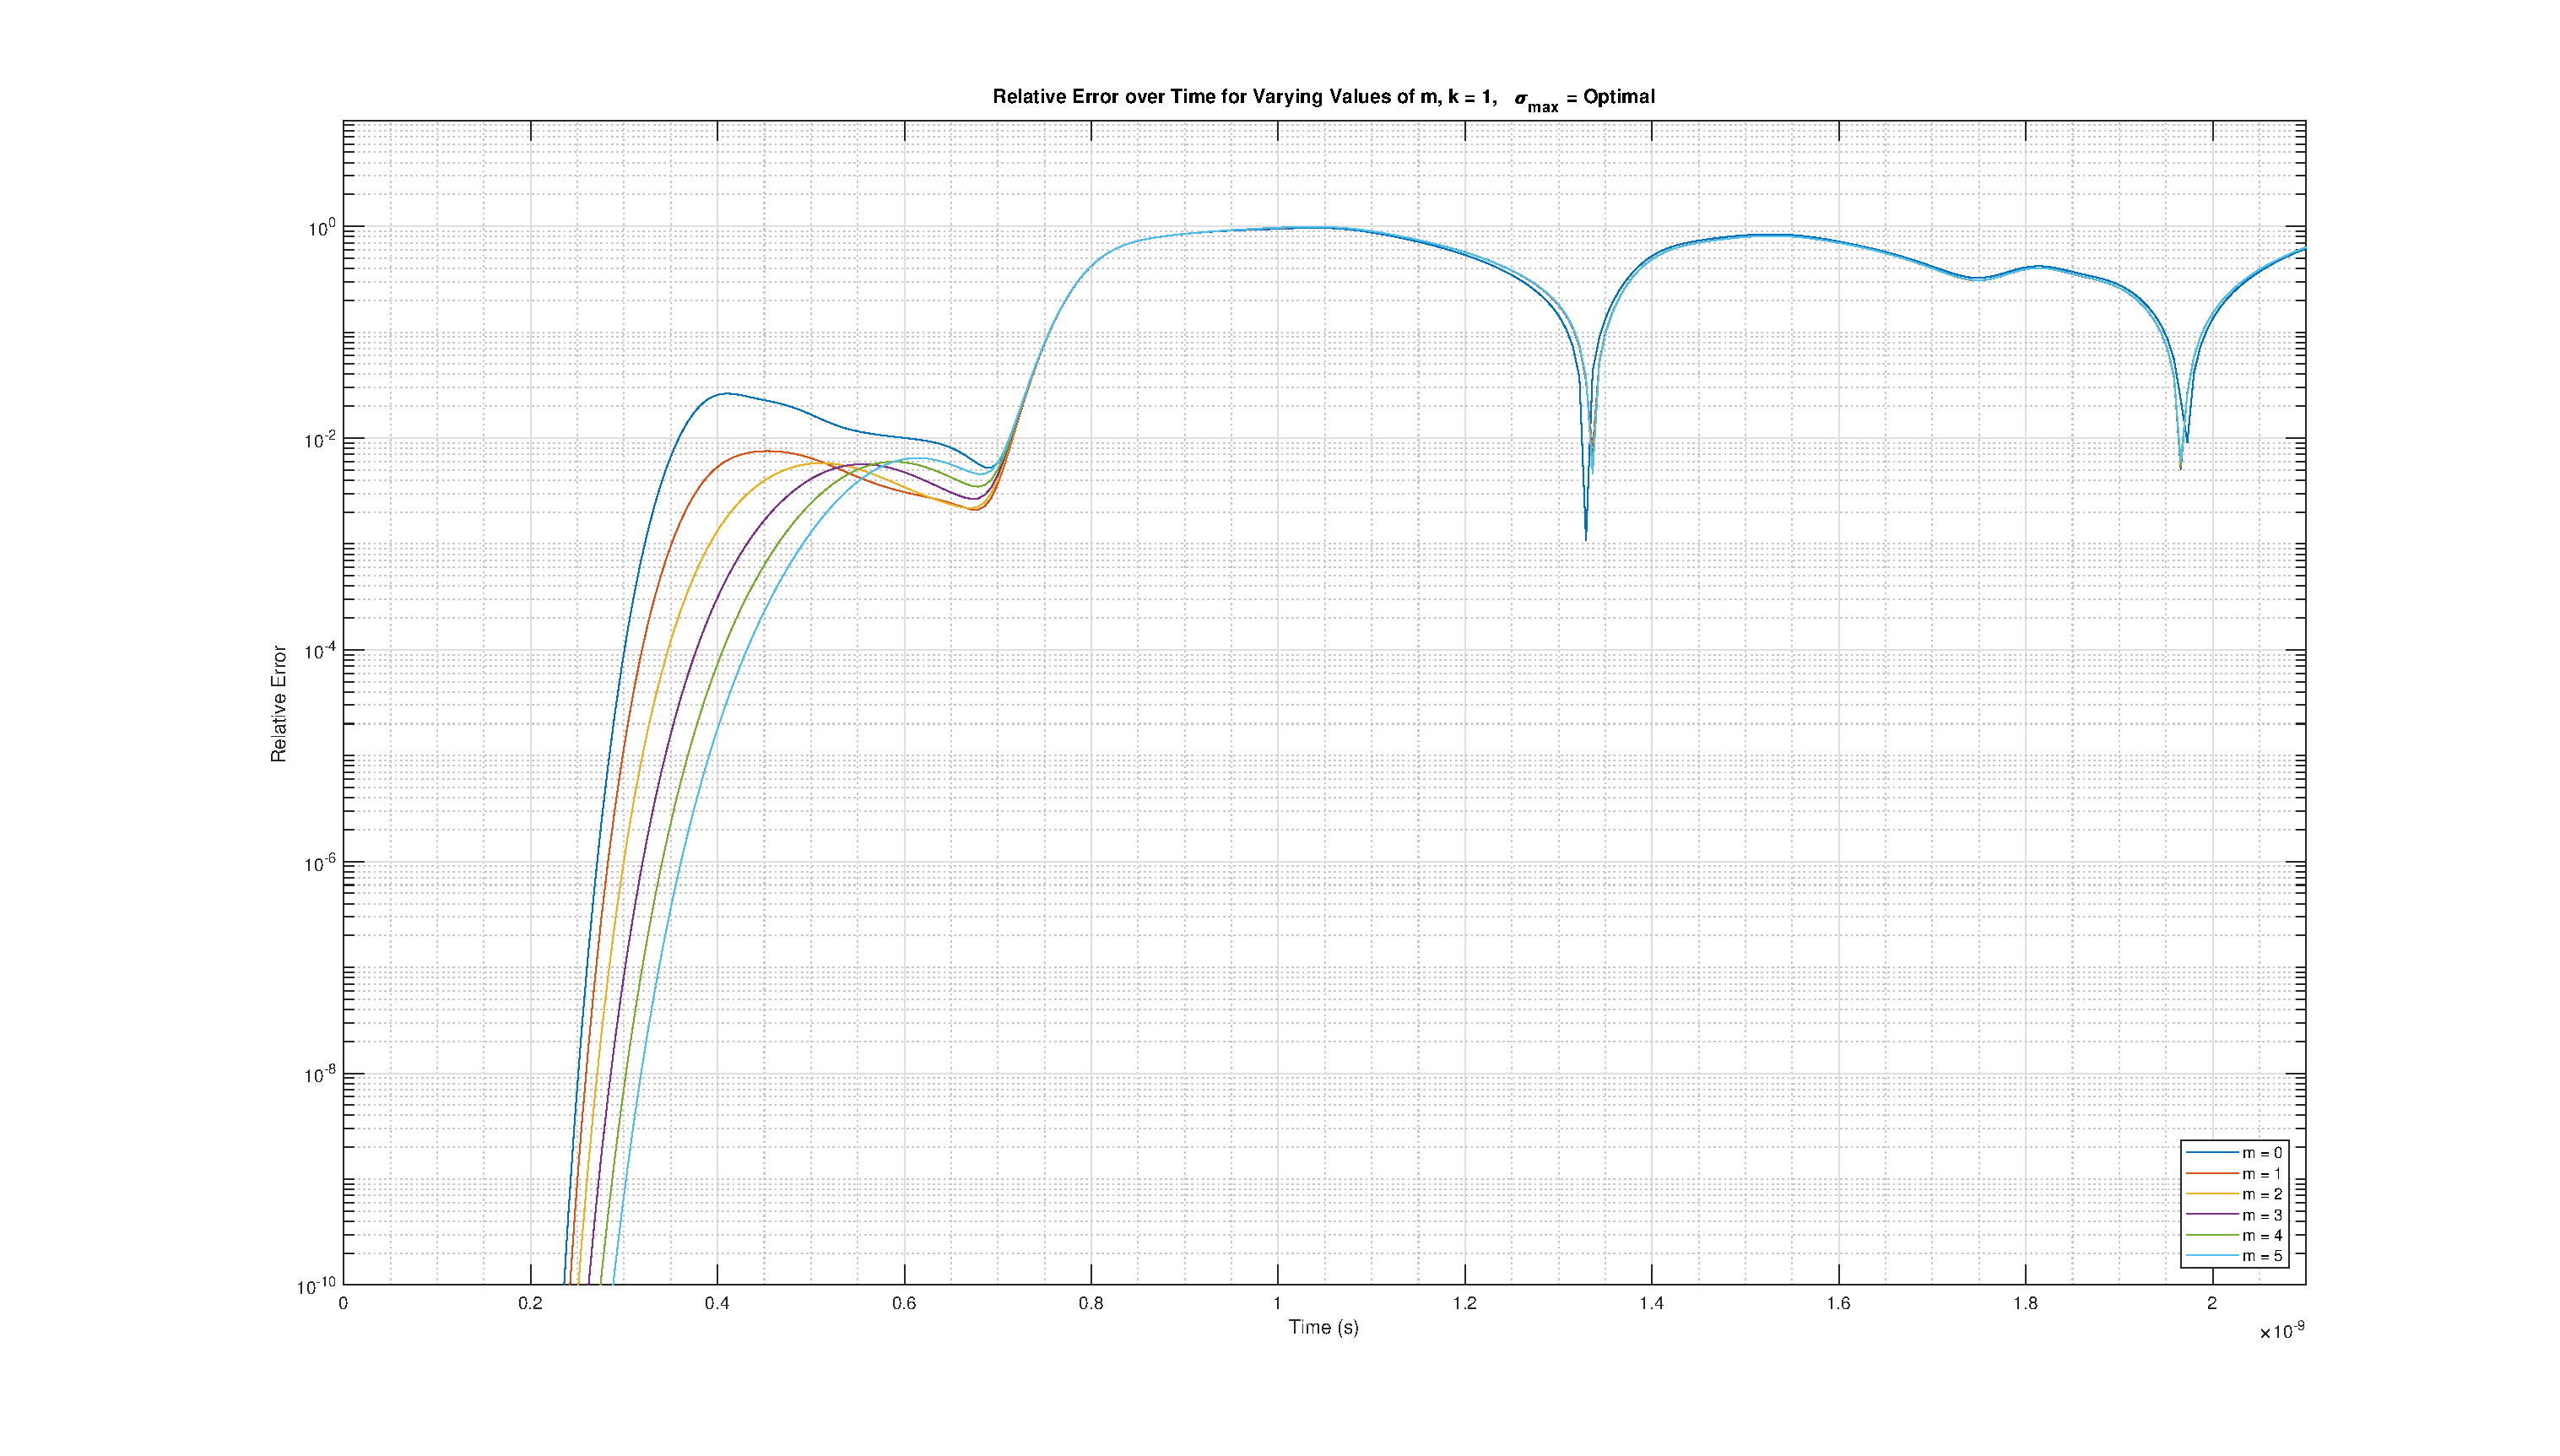
\includegraphics[width=\textwidth]{Rel_Err_m}
  \caption{Plot of Relative Error with respect to time for values of m of 0, 1,
    2, 3, 4, 5}\label{fig:RelErrm}
\end{figure}

\begin{figure}
  \centering
  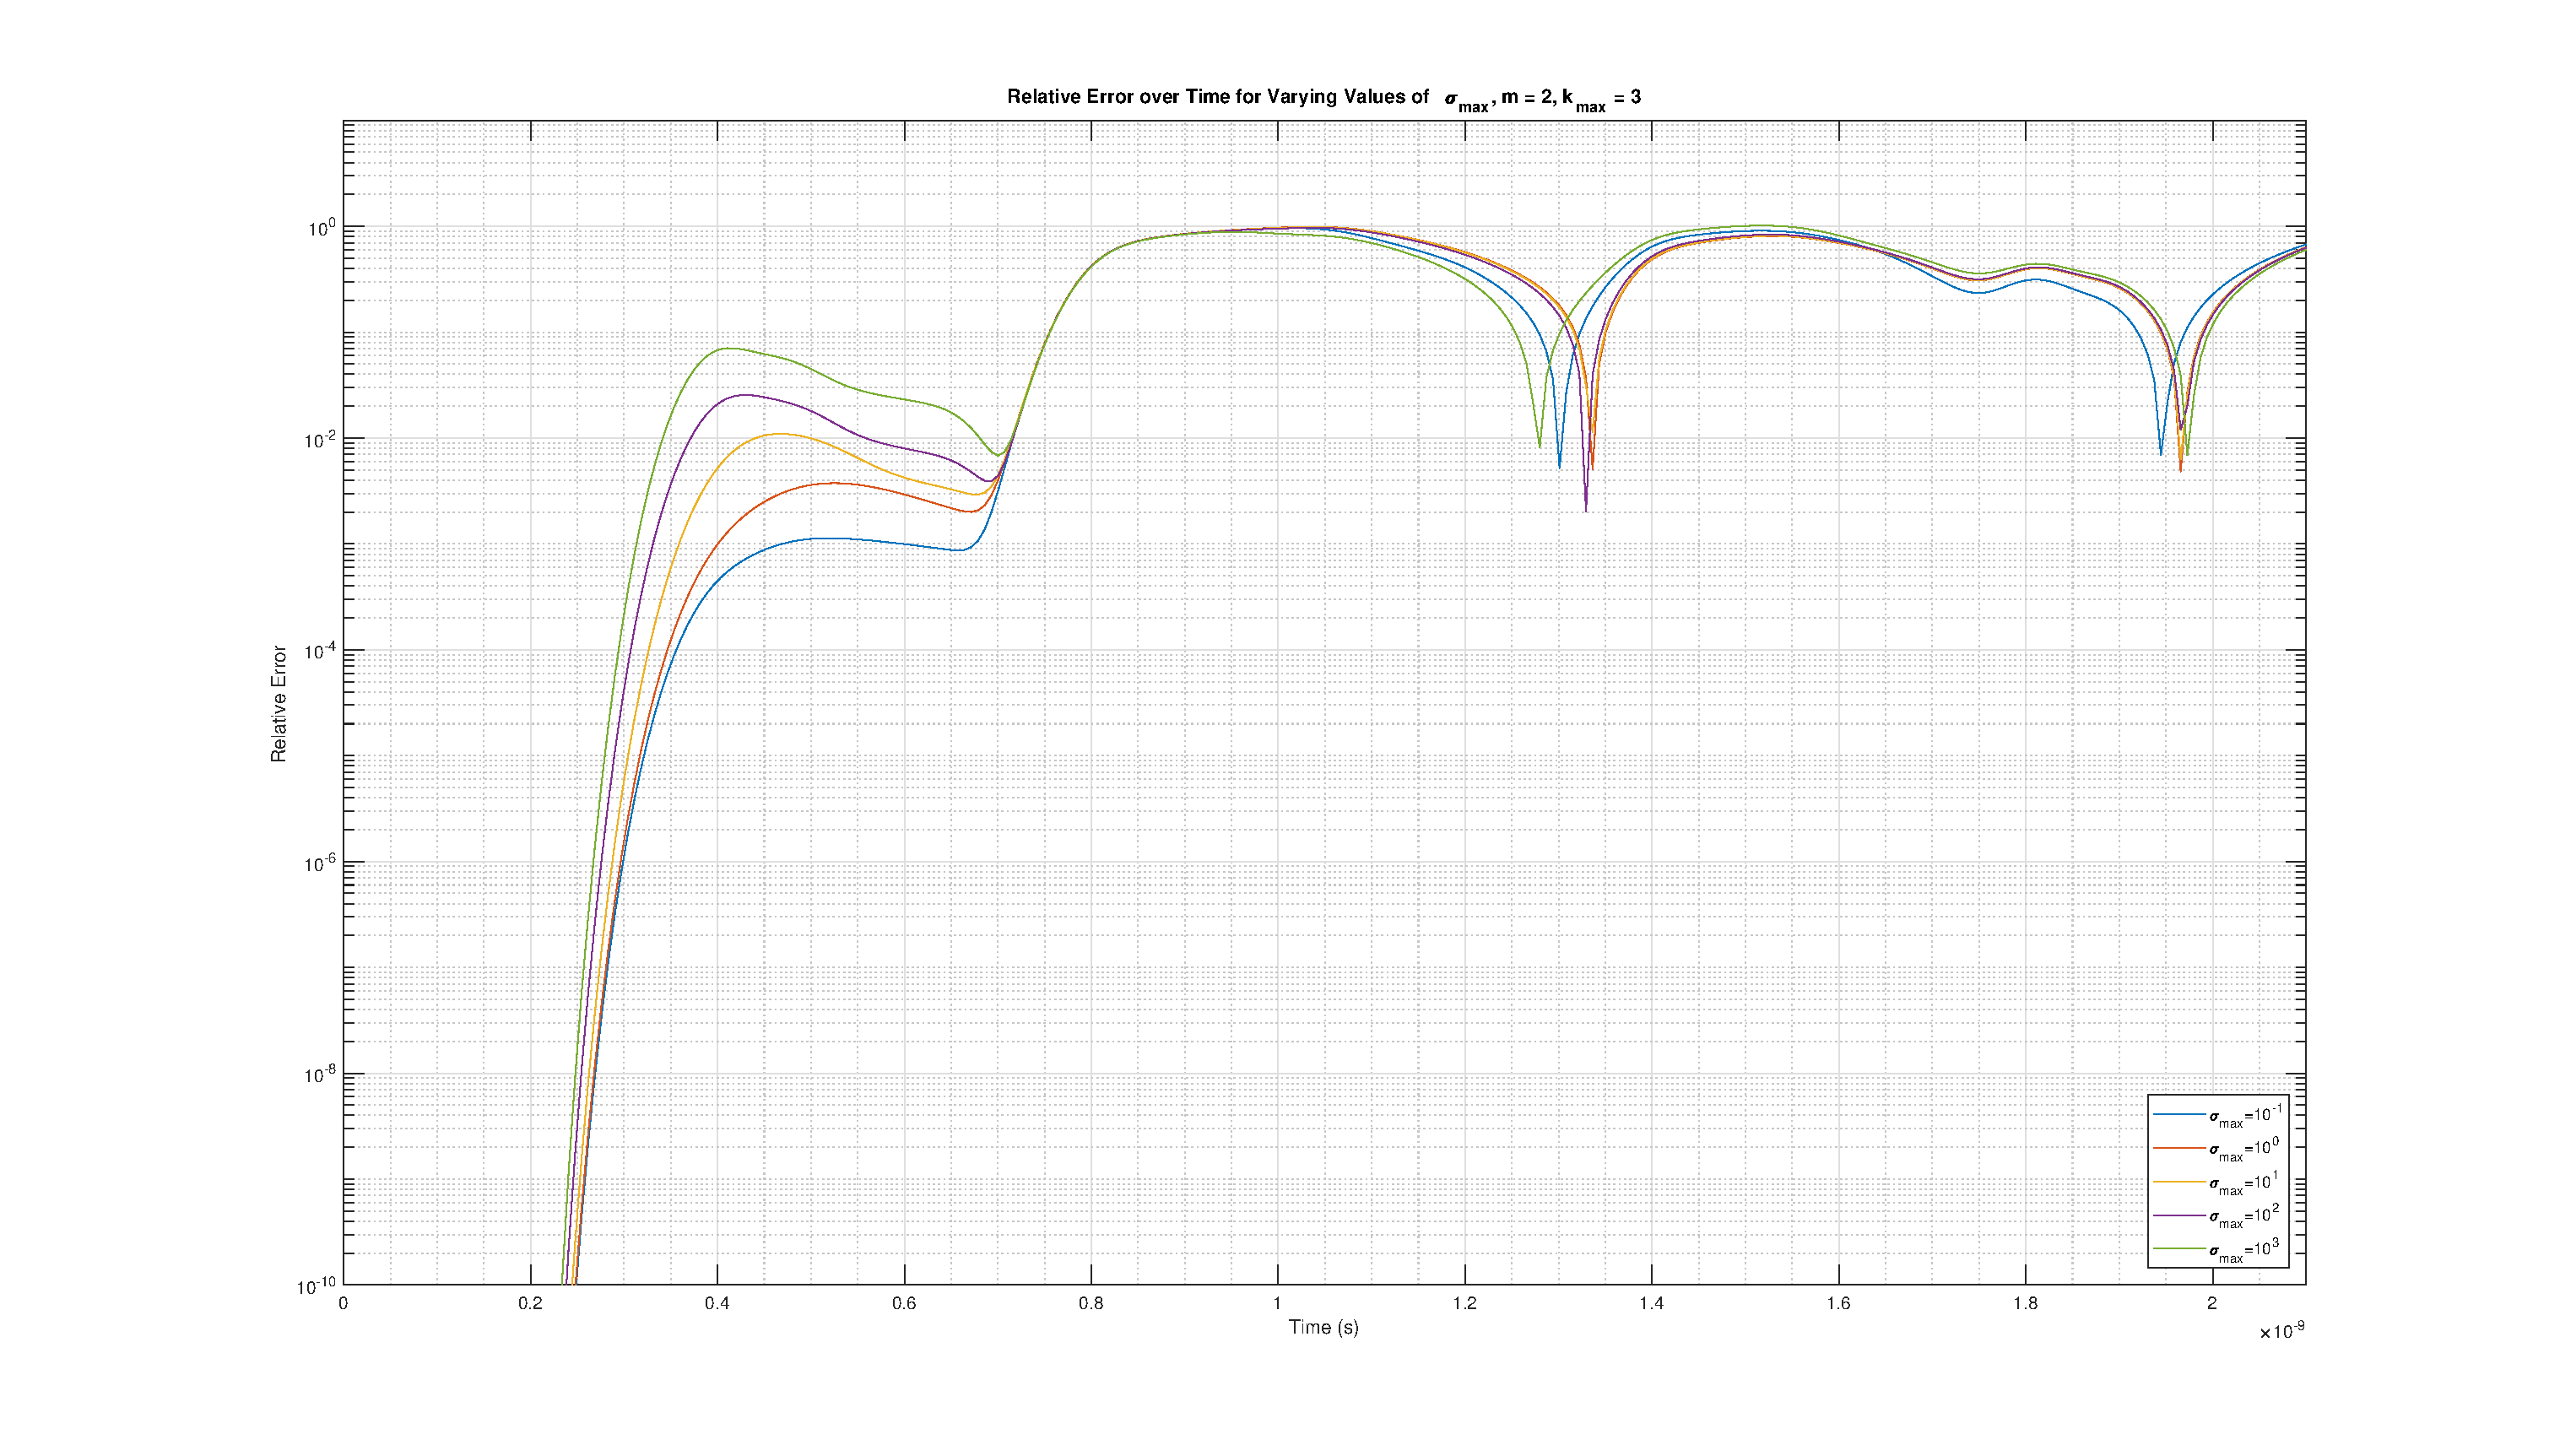
\includegraphics[width=\textwidth]{Rel_Err_SigMax}
  \caption{Plot of Relative Error with respect to time for values of
    \sigma_{max} of 10^{-1}, 10^0, 10^1, 10^2, 10^3, m=2, \kappa{max}=3}\label{fig:RelErrSigmax}
\end{figure}

\section{Bibliography}
Followed Beringer's Derivation in Susan's book - third edition

\end{document}